\subsubsection{Eco Cycle}
In Japan baut das Unternehmen „Giken LTD.“ erfolgreich das automatische Fahrradparkhaus „Eco Cycle“. Es ist das erfolgreichste automatische Parksystem und wurde bereits über 50-mal gebaut. \citev{ginsberg_eco-cycle_2020} Das System kann als Turm oder unterirdisch gebaut werden. Die Funktionsweise ist vergleichbar mit dem „Wöhr Bikesafe“: Das Fahrrad wird in eine Schiene gestellt und mit einem Lagerbediengerät zu einem freien Platz befördert. Es bietet Platz für bis zu 204 Fahrräder.\cite*{ecocycle} Zudem gibt es eine mobile Version des Systems, die leicht auf- und abgebaut werden kann.\cite*{ecocyclemobile}

\begin{figure}[H]
    \centering
    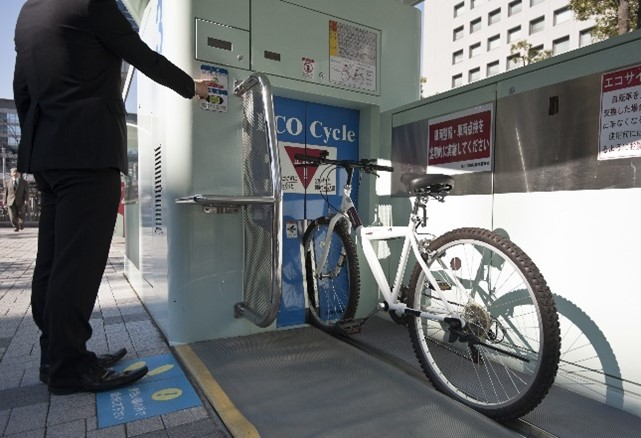
\includegraphics[width=0.5\textwidth]{images/ecocycle.jpg}
    \caption{Eco Cycle \citev{cnn_japans_nodate}}
    \label{fig:ecocycle}
\end{figure}

Die Nachteile des Systems sind ähnlich wie beim „Wöhr Bikesafe“, denn es ist nicht für alle Fahrradtypen oder E-Scooter geeignet und bietet keine alternativen Verwendungszwecke. Die unterirdische Variante ist außerdem nicht überall baulich möglich.